As was noted in chapter~\ref{chp:introduction}, measurements of the \acs{rpnd}
have been mostly limited to the afterglow plasma or time-integrated quantites.
Electric field measurements, either with capacitive probes or nonlinear
wave-mixing, thus far provide the only insight on the development of the
\acs{rpnd}. Though the electric field can be used to estimate electron densities
and reaction rates in the plasma, this requires a number of additional
assumptions such as electron locality, and equilibrium with the applied field.

As a result, there is a lack of reliable information on particle properties of
the \acs{rpnd} during its development. That said, such information is necessary
to confirm the present understanding of how these discharges develop, how they
may be optimized for specific applications, and how to improve existing
numerical simulations. Therefore, a clear need exists for direct measurements of
the \acs{rpnd} particle properties.

Unfortunately, this presents a significant challenge for most traditional plasma
diagnostics. In most situations, the obvious choice would be the Langmuir probe
given its simplicity and ease of implementation. However, the fast variations in
the plasma potential, slow response of the ions, and high collisionality all
preclude this approach \cite{Lieberman2005}. Furthermore, any physical probe
could potentially act as a large perturbation to the very system it is
measuring.

The logical alternative to physical probes is the use of optical diagnostics,
however these have their own associated difficulties. Electrons cannot be
studied by their light emissions because, with the exception of bremsstrahlung
and cyclotron radiation, they do not emit. This leaves the light emitted from
excited atoms. Atomic emission spectroscopy can be used to measure many
different plasma quantities, from electron density, to local electric field
strength. Unfortunately, spontaneous emission can be a slow process compared to
the development of the \acs{rpnd}. For example, the fastest neutral helium
transition in visible wavelengths (3$^3$D$_3$-2$^3$P$_2^\cdot$) has a decay rate
of 14 ns \cite{Ralchenko2011}.

This suggests that instead of waiting for spontaneous emission to occur, it may
be better to use some form of active spectroscopy. Though the added complexity
of a well-characterized light source is undesirable, it allows for several
interesting opportunities. For example, a sufficiently intense laser can be used
to directly interact with the electrons through Thomson scattering. It has a
high spatial and temporal resolution and is able to measure the electron density
and temperature simultaneously \cite{VanGessel2012}. However, the \acs{rpnd} may
have densities well below the interaction limit of $5\times10^{12}$ cm$^{-3}$
\cite{Pai2009}.

If it is not possible to directly interact with the electrons, the next
alternative is interact with the atomic population. Probing of the ground state
is difficult given its large separation from any excited state. Furthermore, the
high densities of the neutral states would completely absorb all incident
radiation, even over short pathlengths (leaving nothing to measure). Instead it
makes more sense to probe an excited atomic state. The lowest lying one is the
triplet metastable (2$^3$S), which resides at 19.82 eV above ground. This
relatively large energy gap assures that no such states will be naturally
present at room temperature. The triplet metastable (and all higher-energy
states in helium) will be populated almost exclusively by energetic electrons.
Therefore, the triplet metastable density is a useful indicator of the electron
energetics in the \acs{rpnd} as it develops. With a sufficiently complex model,
it may even be used to infer properties of the electron population.

Perhaps the most straightforward means by which to measure the triplet
metastable density is with absorption spectroscopy. This approach has a long
history in the study of gas discharges, going back at least six decades
\cite{Phelps1953}. At its most basic, the technique involves illuminating a
plasma with light matching a transition between the metastable, and some upper
level. The amount of transmitted light is then measured with a detector on the
opposite side of the plasma. The amount of transmitted light is proportional to
the metastable density, integrated along the path of the light. As the temporal
bandwidth of this technique is only limited by the time require for the light to
traverse the plasma, it presents a promising approach for particle measurements
during the development of the \acs{rpnd}.

\section{Setup}

Traditionally, the light used in absorption spectroscopy has been supplied by
discharge tubes of same gas as the system under study. Though straightforward,
this approach is limited by the luminosity of the discharge tube, and the fact
that the emitted radiation is isotropic. More recently, Millard et al.\ noted
that diode lasers provide a greatly improved light source for absorption
experiments. The laser light is easily directed and collimated for spatial
selectivity, and has more than sufficient intensity \cite{Millard1998}.
Therefore, it was decided to use a diode laser in the measurement of the triplet
metastable level.

As with the study by Millard et al., the decision was made to study the
transition from the triplet metastable to the 2$^3$P$^\mathrm{o}_{0,1,2}$ state
(a transition wavelength of approximately 1083 nm). This was done for several
reasons. For one, the closest helium transition is over 7 nm away, making it
relatively isolated. In addition, the different levels or values of $J$ are all
within the tuning range of a single diode. As each level has a different
degeneracy, $g$, the strength of absorption varies depending on the selected
level. Thus, the absorption strength can be increased for low densities, or
decreased at high densities, improving the dynamic range of the diagnostic.

The laser used was a distributed feedback laser diode, produced by Toptica,
model LD-1083-0070-DFB-1. The specified linewidth of the laser was 3 MHz, well
below the natural linewidth of the transition at 10.2 MHz. This can be exploited
to directly measure the gas temperature of the system, as will be seen in the
next section. The diode was rated for a total output power of 70 mW, with a beam
size of 1 mm by 3 mm and vertical polarization. The diode was housed in a
Toptica DL DFB housing which incorporated the collimating optics. A Toptica DCC
110 was used to provide current control for the diode laser, and a Toptica DTC
110 was used to control the thermoelectric cooler for the diode.

The layout in figure~\ref{fig:laser}
\begin{figure}
  \centering
  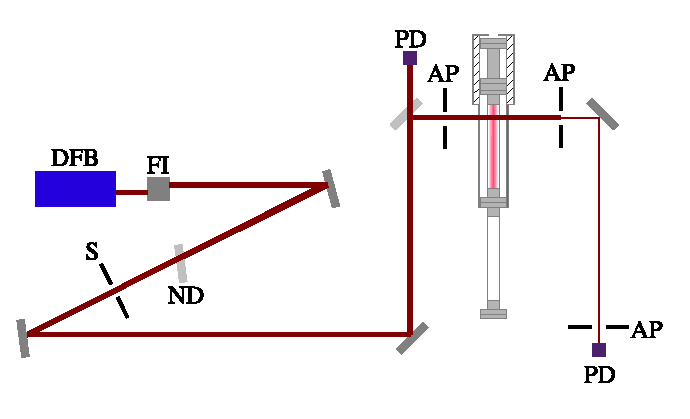
\includegraphics{./chapters/metastables/figures/laser.eps}
  \caption{Optical beam path of the laser in the absorption spectroscopy
  experiment. DFB - Distributed feedback laser diode; FI - Faraday isolator; ND -
  neutral density filter; S - shutter; PD - photodiode; AP - aperture.}
  \label{fig:laser}
\end{figure}
reflects the optical beam path used in the absorption experiment. The laser
light is produced by the distributed feedback laser diode (DFB). It then enters
an Electro-Optics Technology, Inc. Faraday isolator (FI) which prevents
back-reflections from entering the diode. Without the isolator in place, such
back-reflections can cause mode-hopping, resulting in unreliable tuning. The
laser intensity is then reduced by a neutral density filter (ND). After which,
the laser passes through a Vincent Associates electronic shutter (S). Then, the
beam is split by a Thorlabs BSF10-C beam sampler at a 45$^\circ$ angle. This
reduced the laser intensity below the saturation intensity (0.45 mW/cm$^2$) of
the transition. The beam was collimated with two apertures (AP) on both sides of
the discharge apparatus. The beam exiting the apparatus was then sent through a
final aperture to filter nearly-colinear plasma emissions before it was coupled
into an optical fiber by a Thorlabs F240SMA-780 collimation package.

Behind the beam sampler was a Thorlabs DET300 germanium photodiode. The signal
from this photodiode was terminated at 1 M$\Omega$ and used to monitor the beam.
The opposite end of the optical fiber was affixed to a Thorlabs DET410 InGaAs
photodiode. The photodiode signal was amplified by a Femto HVA-200M-40-B voltage
amplifier before being sent to the oscilloscope. The time resolution of the
metastable measurements was determined by the InGaAs photodiode which had a
specified rise time of 5 ns.

In order to measure the absorption of the laser, it was first necessary to tune
the laser to the correct wavelength. This matter was complicated by the lack of
a wavemeter with sufficient precision and accuracy. As a result, a signal
generator was used to sweep the laser current so as to cover a frequency range
of 40 GHz while the plasma was operating. The temperature of the diode was then
slowly adjusted until absorption peaks corresponding to the 2$^3$S$_1$ -
2$^3$P$_{0,1,2}^\mathrm{o}$ transition were observed in the output of the InGaAs
photodiode. This allowed the laser current to be tuned to coincide with the
desired transition and provided a rough conversion between changes in the diode
current and changes in the laser wavelength. A more accurate measurement of this
relation was made with a CVI Melles Griot ET-25.4-10.00-30, solid dielectric
etalon. It was found that a temperature of 36$^\circ$ C and a current of 63 mA
produced resulted in an output wavelength of approximately 1082.9 nm and the
conversion between diode current and wavelength was $0.6067$ mA/GHz.

As described in chapter~\ref{chp:experiment}, data acquisition was handled by a
LabView program, connected to the oscilloscope by a GPIB cable. The auxiliary
outputs of the SRS SR850 lock-in amplifier were used to adjust the diode laser
current (via the DCC 110 module), and to trigger the electronic shutter. One of
the auxiliary inputs of the lock-in amplifier was used to read out the pressure
from the pressure controller.

Data were acquired for a range of pressures from 0.3-16.0 Torr, and at three
axial locations: 5.08, 12.7, and 20.32 cm, relative to the glass-metal seal of
the anode. In reference to their location relative to the gas inlet these will
be referred to as the `upstream', `midstream', and `downstream' locations,
respectively. For each combination of location and pressure, absorption spectra
were measured over $\pm3.85$ GHz relative to the nominal transition frequency of
the 2$^3$S$_1$-2$^3$P$_0^\mathrm{o}$ transition at intervals of 154 MHz. The
absorption spectra were measured for time domains of $-300$-$1700$ ns relative
to the voltage pulse. Additional measurements were made at the midstream
position of the metastable densities from $-88$-$700$ $\mu$s in order to
investigate the loss mechanisms of the metastables.

The broadband electronic noise emitted by the fast pulses was a persistent issue
and presented one the greatest challenges to measurements during the \acs{rpnd}
development. As described above, the InGaAs photodiode was removed from the
immediate area surrounding the discharge by the use of an optical fiber. The
optical fiber was routed through a small opening in a grounded metal box where
both the photodiode and the voltage amplifier resided. In addition, the DC power
supply of the voltage amplifier was connected to an outlet on a Tripp-lite
Isobar intended to provide additional isolation. The photodiode was connected
directly to the input terminal of the amplifier, while the amplifier was
connected to a BNC bulkhead adapter by a 10 cm length of RG 50/U. The final
connection to the oscilloscope was made by an additional 10 cm length of RG
50/U, running from the BNC bulkhead connection.

Figure~\ref{fig:transmitted}
\begin{figure}
  \centering
  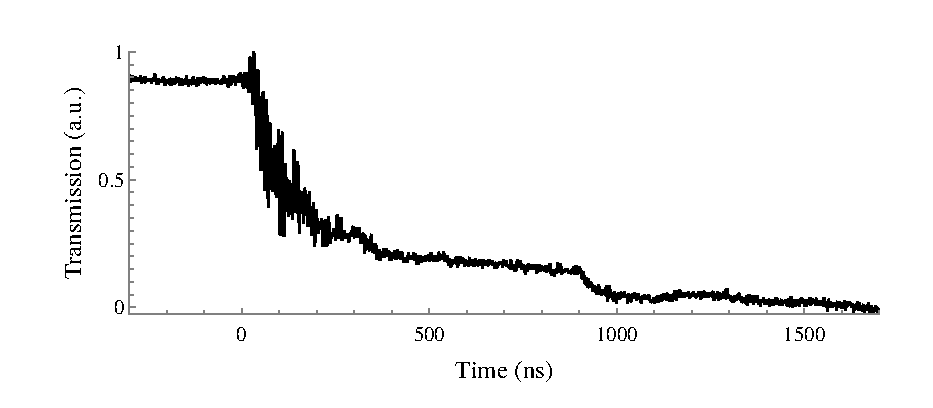
\includegraphics{./chapters/metastables/figures/transmitted.eps}
  \caption{Measurement of the transmitted laser light at the nominal transition
  wavelength at 4.0 Torr of helium.}
  \label{fig:transmitted}
\end{figure}
shows the transmission signal measured at the nominal transition wavelength for
a \acs{rpnd} in 4.0 Torr of helium. The signal is an average of 200 independent
pulses. Further sampling had no appreciable effect on the waveform. As can be
seen, despite the efforts to limit the electrical interference, there is still a
substantial amount of noise present in the transmission signal. This is most
noticeable in the large ringing which occurs for the first 200 ns after the
voltage pulse. Without any kind of compensation, it would be impossible to
obtain reliable measurements of the transmission signal.

\section{Absorption Analysis}

The noise produced by the \acs{rpnd} was relatively consistent between pulses as
well as over the duration of each experiment. As a result, it was possible to
correct for the electrical noise and any spontaneous plasma emissions by
measuring the signal from the photodiode in the absence of the laser and
subtracting this from the signal with the laser. The acquisition process
proceeded as follows:
\begin{enumerate}
  \item Set desired laser wavelength.
  \item Wait 5 s for laser output to settle.
  \item Acquire 200 waveforms from photodiode.
  \item Close shutter.
  \item Acquire 200 waveforms from photodiode.
  \item Repeat
\end{enumerate}
The effect of this subtraction can be seen in figure~\ref{fig:contours}
\begin{figure}
  \centering
  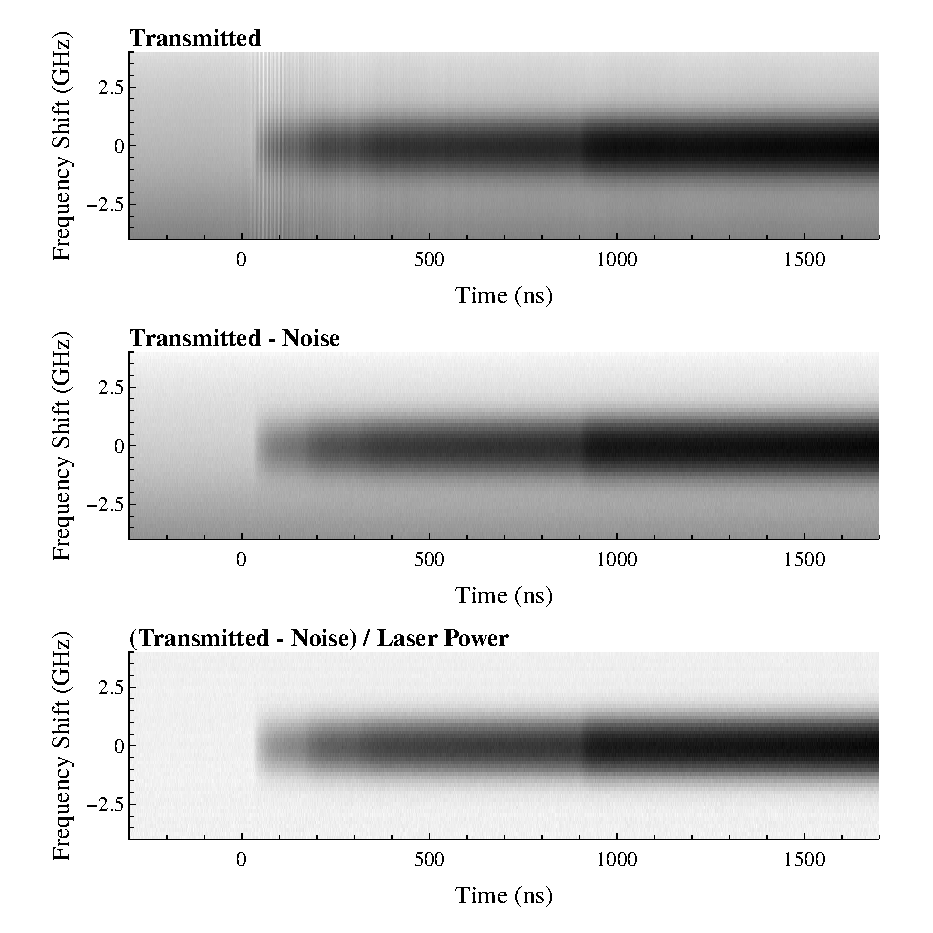
\includegraphics{./chapters/metastables/figures/contours.eps}
  \caption{Heatmaps of the transmitted laser signal for the 4.0 Torr condition at 
  various stages of post-processing.}
  \label{fig:contours}
\end{figure}
where the top heatmap shows the initial set of acquisitions with the laser on,
and the middle heatmap shows the transmitted signal with the noise subtracted.

As the wavelength of the laser diode changed, so did the output power. The
produces the gradient-like appearance of the top two plots in
figure~\ref{fig:contours}. In order to obtain a measurement of the unattenuated
laser power, the above acquisition procedure was repeated with the plasma off
for each operating condition. This made it possible to correct for the varying
laser power and to produce properly scaled transmission spectra.

These transmission spectra were then analyzed using a transmission model based
on the absorption cross sections described in chapter~\ref{chp:theory}. In a
one-dimensional system, the change in intensity of an incident photon field
(below the saturation limit), can be expressed as
\begin{equation}
  \frac{dI(x, \omega)}{dx} = -\sigma(\omega) N(x) I(x, \omega)
\end{equation}
where $I$ is the intensity of the photon field as a function of distance $x$,
$\omega$ is the frequency of the photons, $N$ is the density of the interacting
species, and $\sigma$ is the interaction cross section. This equation has the
simple solution,
\begin{equation}
  T(\omega) = \frac{I(x, \omega)}{I_0(\omega)}
            = \exp\left[-\sigma(\omega) \int_0^x N(x') dx'\right],
  \label{eq:transmitted}
\end{equation}
where $T$ is the transmitted intensity fraction, and $I_0$ is the initial
intensity of the photon field. The absorption can be trivially obtained from the
equation $A(\omega) = 1 - T(\omega)$.

For the purpose of analyzing the absorption, a quantity called the
line-integrated density will be defined. This is simply, $\nint = \int_0^x
N(x')dx'$. Equation~\ref{eq:absorb} can be used to determine the absorption
cross section. However, this requires that a lineshape be specified. If
possible, it is preferable to select either a purely Gaussian or purely
Lorentzian lineshape as the Voigt profile (equation~\ref{eq:voigt}) is
accompanied by a significantly larger computational cost. This can be determined
by a comparison of the relative widths of the different broadening mechanisms.
For a temperature of 300 K and a pressure of 8.0 Torr, it is found that $\dwd =
1.7$ GHz and $\dwa = 0.21$ GHz. Because neither broadening mechanism is
significantly dominant, the choice was made to analyze the data with a Voigt
profile, despite the added computational cost.

Equations~\ref{eq:transmitted},~\ref{eq:absorb}, and~\ref{eq:voigt} can be
combined to form a model equation for the transmitted spectrum. It can be seen
that only two unknowns exist: the gas temperature, $T_g$, and the
line-integrated density, $\nint$. For each time step, this model equation was
matched to the measured spectrum using the Levenburg-Marquardt algorithm
\cite{Marquardt1963} as implemented by the SciPy library \cite{Jones2001}.
During the matching process, it was observed that the diode current for which
absorption was optimized would shift over time. This was assumed to be the
result of small, long-term variations in the diode temperature that were not
adequately compensated for by the temperature control system. This corresponded
to a frequency drift of $\pm60$ MHz between experiments. For each experiment,
this frequency offset was measured for the spectrum with the largest absorption
signal and was then used to correct the analysis of all other spectra.

\section{Results}

The matching algorithm proved robust enough to automatically match the
transmission spectrum at each time step with no user intervention.
Figure~\ref{fig:matching}
\begin{figure}
  \centering
  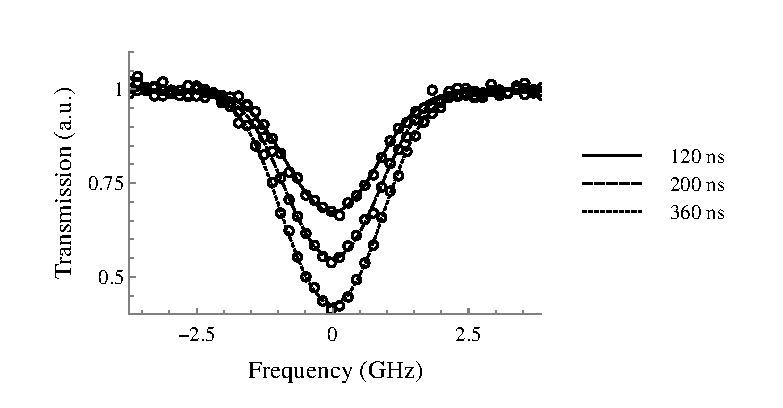
\includegraphics{./chapters/metastables/figures/matching.eps}
  \caption{Comparison of the measured transmission profile (open symbols) and
  the computer-generated matches for at several different times for the 4.0 Torr
  operating condition.}
  \label{fig:matching}
\end{figure}
shows three examples of the measured transmission spectra along with the
computer-generated matches. The measure data far from the peak coincide almost
perfectly with an unabsorbed signal. In addition, the spectrum at 120 ns shows
no evidence of the noise caused by the discharge. The variation in the baseline
transmission signal is approximately 0.02. This sets a minimum line-integrated
detection limit of approximately $3.0 \times 10^{14}$ m$^{-2}$, though the
actual value will depend to some extent on the pressure and temperature.

\subsection{Temperatures}

The temperatures calculated for the metastables from the laser-absorption
spectroscopy are shown in figure~\ref{fig:temperatures}.
\begin{figure}
  \centering
  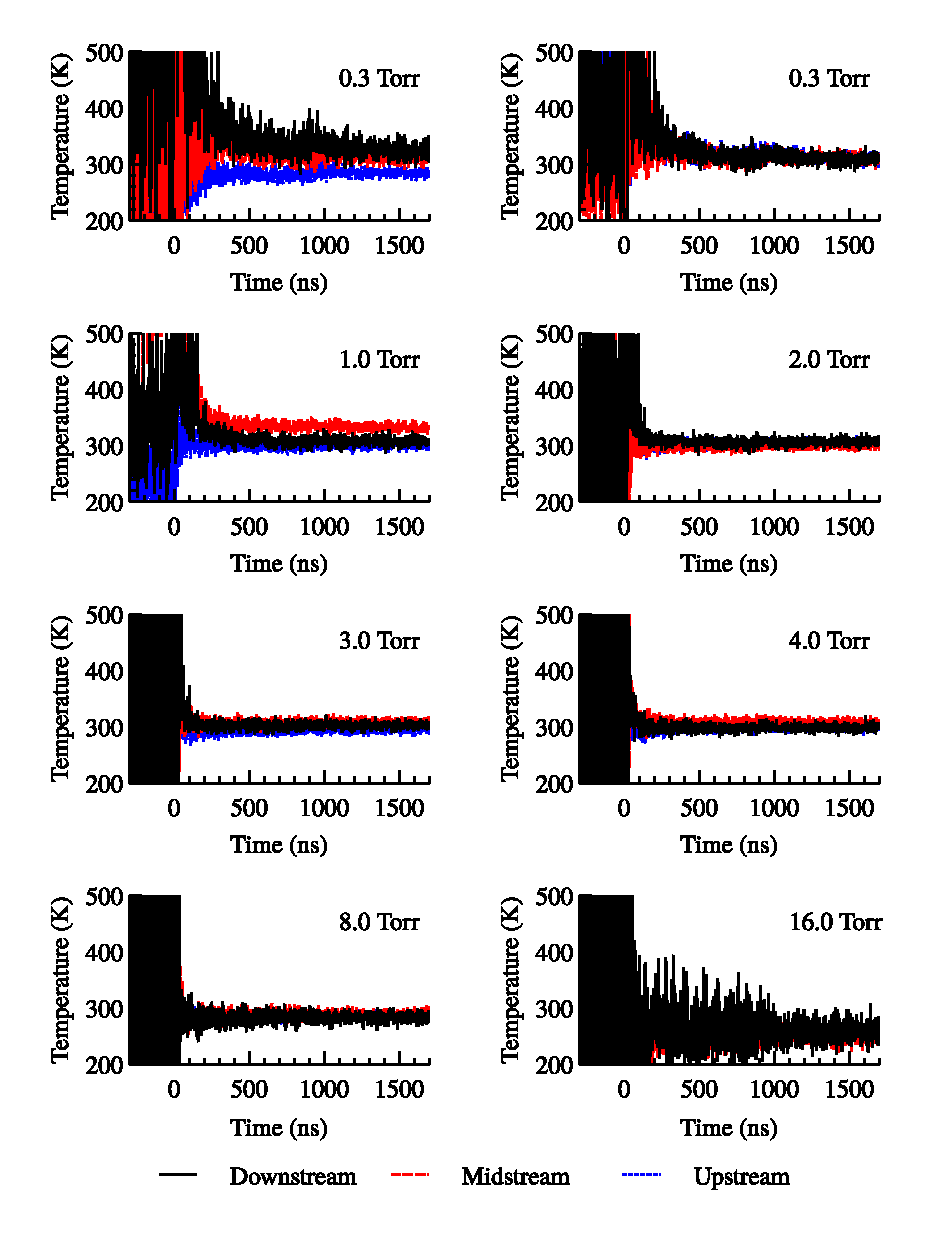
\includegraphics{./chapters/metastables/figures/temperatures.eps}
  \caption{Plot of the gas temperatures at each of the operating
  pressures and each axial location as a function of time.}
  \label{fig:temperatures}
\end{figure}
Prior to the pulse, the temperature estimates are subject to large variations.
This is a result of the low metastable densities which precede the pulse.
Without a substantial metastable population to work with the matching algorithm
has difficult discriminating between a combination of low temperatures and low
densities (a small narrow absorption spectrum) versus high temperatures and high
densities (a very broad absorption spectrum).

It is not possible to precisely calculate the error for the matching process at
each time step, however it is possible to estimate the standard deviation. In
all cases, the estimated standard deviation is less than 10 K by the end of the
measurement period. Based on the covariance estimates, there appear to be no
meaningful trends over the measurement period or between measurement locations.

In order to more clearly compare the temperatures at the different operating
conditions, the results for each location were combined and averaged over the
final 200 ns. This was then plotted with respect to the energy deposition
calculations from chapter~\ref{chp:experiment}, divided by the gas density.
The results are shown in figure~\ref{fig:tvp}.
\begin{figure}
  \centering
  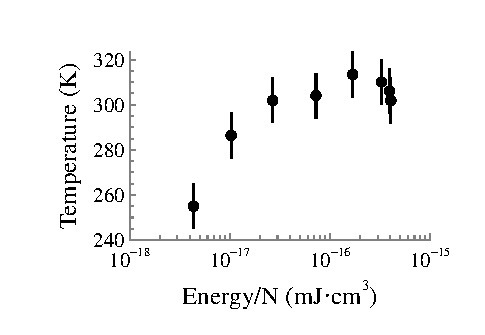
\includegraphics{./chapters/metastables/figures/tvp.eps}
  \caption{Plot of the average gas temperature as a function of deposited
  energy.}
  \label{fig:tvp}
\end{figure}
For the majority of operating conditions, there is little to know statistical
difference between the results and room temperature. The one exceptional
condition is the 16.0 Torr operating condition at 4.33$\times10^{-18}$
mJ/cm$^3$ with a mean temperature of 255 K. As the glass of the discharge tube
as at room temperature for all experimental conditions, this does not appear to
be a reasonable result for the temperature. Examination of the individual
absorption spectra did not reveal any obvious errors in the calculated matches.
However, as will be seen later, the metastables were the least dense at 16.0
Torr. This, coupled with the large variation of the temperatures in
figure~\ref{fig:temperatures} suggest that the standard deviation is potentially
lager than 10 K. Such a situation would explain the unreasonable temperature
obtained for this condition.

The literature provides only a limited number of direct temperature measurements
for similar systems. The most similar work in appears to be that of Walsh et al.
\cite{Walsh2010} in which the temperature of a \acs{rpnd} in helium with a small
admixture of oxygen was measured by optical emissions. The geometry consisted of
two cylindrical steel electrodes separated by 2 mm with a single dielectric
barrier between the two, a gas flow rate of 5 slm, at atmospheric pressure.
Temperatures ranged from 300-340 K, depending on the average power dissipated in
the plasma. Walsh et al. suggest that the observed temperature increase is a
result of Joule heating, that is, heating of the gas as a result of electrons
colliding with neutral particles. As the neutral collision frequency scales
linearly with pressure, this would certainly explain the negligible heating
observed in figure~\ref{fig:tvp}. The presence of a large fraction of a
molecular gas (oxygen) presents another potential heating mechanism when
dissociation occurs, called Franck-Condon heating, and excitation of rotational
and vibrational states which relax to translational energy
\cite{Kiehlbauch2003}.

Other experiments have demonstrated minimal gas heating, as in the case of
plasma bullets \cite{Laroussi2005, Lu2006}, while others have measured final
temperatures ranging from 400-1000 K \cite{Pai2009, Popov2011, Zuzeek2010} (see
appendix~\ref{chp:oes} for detailed study in air). From the available
literature, measurable heating only appeared to coincide with measurements of
\acs{rpnd}s in molecular gases. This emphasizes the importance of the heating
mechanisms mentioned earlier and likely plays a large role in the nonthermal
nature of the atmospheric pressure helium plasmas.

Recent simulations and rate calculations \cite{Takashima2011, Aleksandrov2007}
have provided estimates of the electron temperature in the range of 10-20 eV. As
a result, all of the discharges mentioned are very much nonthermal in nature.
That said, the negligible heating in the helium \acs{rpnd} studied here presents
a significant advantage for many applications, as even the moderate temperature
increases in molecular discharges can threaten material integrity. For example,
most commercial polymers are only rated to 300$^\circ$ C, making them
susceptible to damage without careful thermal management.

\subsection{Line-integrated Densities}

As described in the analysis section, the laser-absorption spectroscopy also
yielded the line-integrated metastable densities. Figure~\ref{fig:metastables}
\begin{figure}
  \centering
  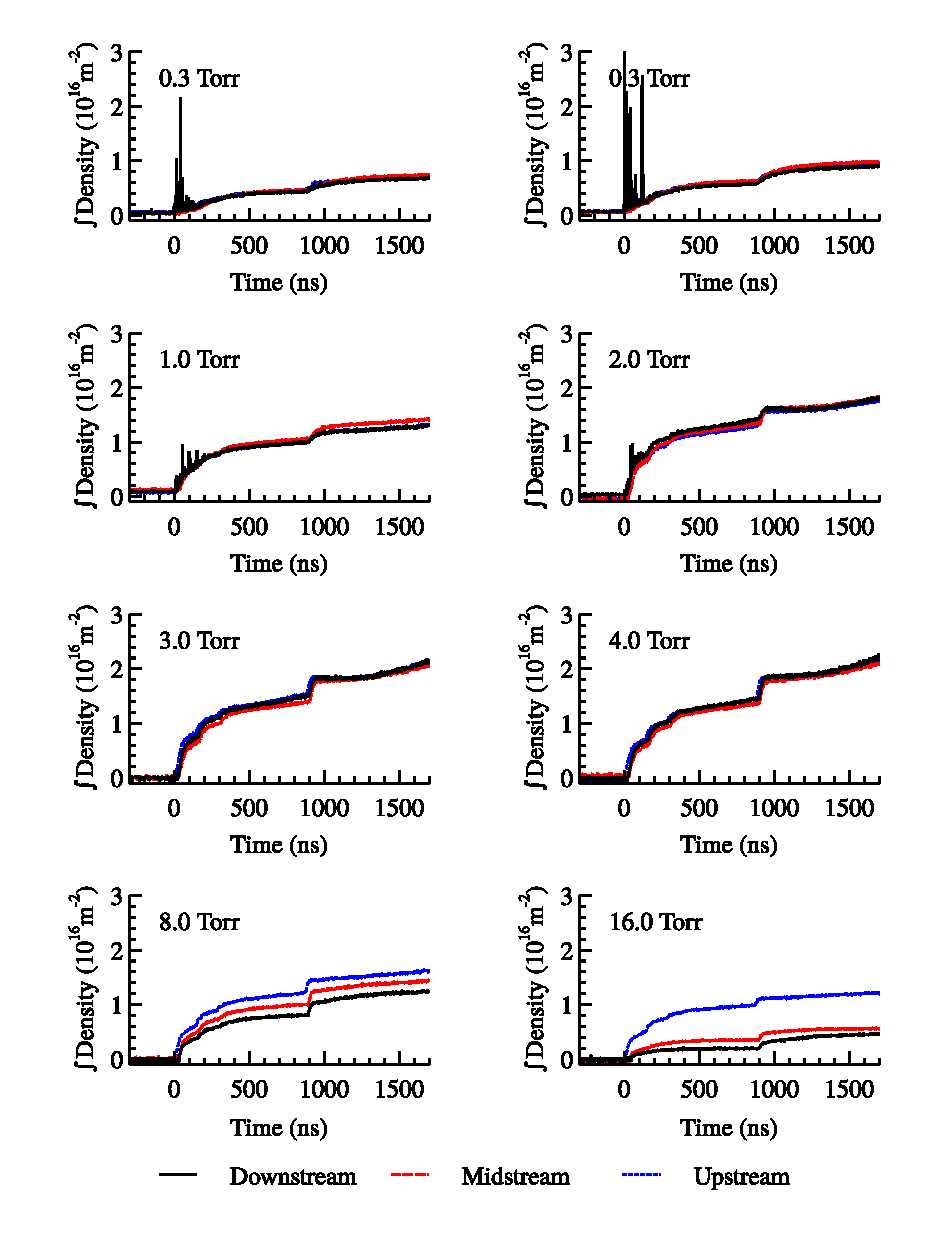
\includegraphics{./chapters/metastables/figures/metastables.eps}
  \caption{Plots of the line-integrated metastable densities at each of
  the operating pressures and each axial location as a function of
  time.}
  \label{fig:metastables}
\end{figure}
features the metastables dynamics for each operating pressure and at each
location. Similar to the temperature measurements, there is a substantial
uncertainty during the pre-pulse period for pressures greater than 1.0 Torr.
However, for 1.0 Torr and below, there are detectable populations of triplet
metastables, around $7\times10^{14}$ m$^{-2}$. These excited atoms are the
remnants of the previous pulses which have not been destroyed. Despite the
efforts made to limit the noise in the signals, there is a significant number of
erroneous data points at pressures below 3.0 Torr in the downstream
measurements. The reason for this is not apparent. The only change was the
position of the mirror directing the transmitted laser light into the fiber
coupler. That is, the position of the photodiode did not change between
measurements. 

The population of the metastable states exhibits several small bursts, in short
succession, after the pulse at about 140 and 270 ns. The timing of these rapid
rises in density correlate to the arrival of pulse reflections. This suggests
that the even after the plasma has formed, additional pulses are still able to
deposit a significant amount of energy in the plasma. In all reported cases, the
final metastable density grew to exceed twice the density after the first pulse.
This appears to contradict the predictions made by the one-dimensional drift
models of Adamovich et al. \cite{Adamovich2009} and Nikandrov et al.
\cite{Nikandrov2008} which stated that little energy is coupled into the plasma
after breakdown occurs. In addition to the smaller bursts in density, another
can be noted at about 900 ns which corresponds to the double-pulsing observed in
the current-voltage characteristics of chapter~\ref{chp:experiment}.

By 200 ns after the pulse, the estimated standard deviation in all cases is
approximately $2\times10^{14}$ m$^{-2}$. Based on this, it can be concluded that
the metastable populations had no significant axial dependence below 8.0 Torr.
However, both 8.0 and 16.0 Torr conditions showed notable differences in the
metastable population as a function of distance from the anode. As might be
expected, the upstream location (closest to the anode) has a high metastable
population than the other two. At 16.0 Torr, the line-integrated density at 16.0
Torr was over twice that of either location.

This behavior is reminiscent of that observed by Vasilyak et al.
\cite{Vasilyak1994} in \acs{fiw} devices. It was noted that the electric field
of the wave would attenuate with distance. In order to interpret this, they
considered the wave to consist of two components: a moving ionization front with
a finite width, and the plasma left in its wake. They state that the plasma,
with its finite conductivity, will have some voltage drop across it, and as it
grows, this drop increases. As a results the voltage drop across the ionization
front can never be greater than the overall potential applied to the system and
is constantly diminishing as it moves away from the energized electrode. If
true, this behavior would be associated with a reduction in the rate of
metastable generation in the front, thus explaining the high pressure data in
figure~\ref{fig:metastables}.

\subsection{Metastable Destruction}

In addition to the fast metastable dynamics, measurements were made of the
long-term trends in metastable population. As previously mentioned, afterglow
measurements such as these are less subject to the noise and bandwidth
limitations of the short timescale measurements. This makes it possible to
obtain relatively clean and precise values for the metastable densities.
However, without the applied electric field the nonequilibrium dynamics of the
system rapidly disappear. Therefore, these measurements do not provide much
insight on the development of the \acs{rpnd}.

That said, a large body of work has been conducted on helium afterglow
discharges, which makes this regime attractive as a point of comparison.
Furthermore, these measurements include the peak metastable populations for each
operating pressure (which are missing from figure~\ref{fig:metastables}). The
peak metastable densities and the lifetime of the metastable populations are of
interest as they can produce charged particles through Penning ionization of
each other or impurities. This extends the ionization period in rare gas
\acs{rpnd}s well past the voltage pulse itself. Also, as seen in
figure~\ref{fig:grotrian}, all excited states in the triplet manifold will
eventually decay to the triplet metastable level. Thus, a substantial portion of
the energy deposited in the plasma is contained in this one level.

Figure~\ref{fig:long}
\begin{figure}
  \centering
  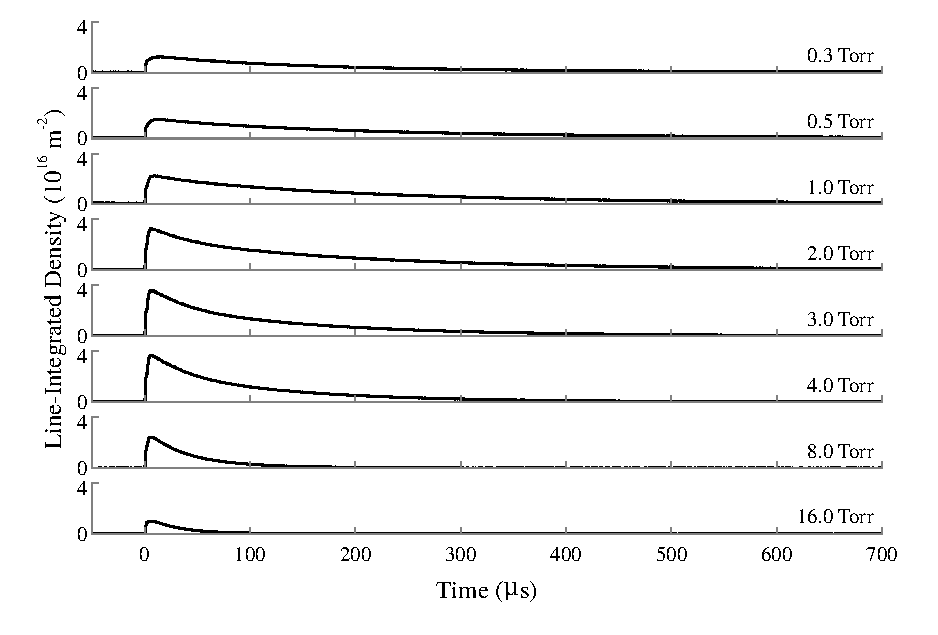
\includegraphics{./chapters/metastables/figures/long.eps}
  \caption{Measurements of the long-duration metastable density trends.
  Exponential fits are indicated by the dotted lines.}
  \label{fig:long}
\end{figure}
contains logarithmic plots of the metastable populations for each operating
condition, all measured at the midstream location. In addition, an exponential
function was fit to the tail of each trend, represented by the dotted line. On
these time scales, the destruction of metastables in the \acs{rpnd} apparatus
can be described by four different mechanisms: diffusion, Penning ionization of
impurities, Penning ionization between metastables, and three-body collisions
resulting in helium dimer formation. All processes with the exception of the
Penning ionization between metastables have an exponential dependence, thus any
deviation from an exponential decay is likely a result of this process
\cite{Deloche1976}.

As can be seen, a number of the decay curves deviate from a strictly exponential
decline. This deviation appears to be more substantial at the lower pressures,
as by the 16.0 Torr case the decay appears strictly exponential. Penning
ionization is proportional to the square of the metastable density, thus it
would be expected that the deviation from the exponential decay would be most
severe for the highest metastable densities. However, per
figure~\ref{fig:peaknm},
\begin{figure}
  \centering
  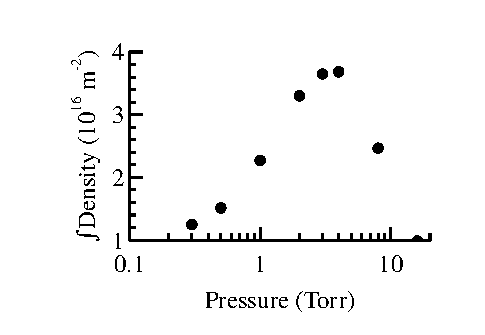
\includegraphics{./chapters/metastables/figures/peaknm.eps}
  \caption{Peak line-integrated metastable densities as a function of pressure.}
  \label{fig:peaknm}
\end{figure}
this suggests that the deviation from the exponential decay should be lessened
at the lower pressures, contrary to what was observed.

Ultimately, the behavior of the metastable populations in the afterglow can be
best understood by a comparison of the depopulation rates for each process.
Figure~\ref{fig:decay}
\begin{figure}
  \centering
  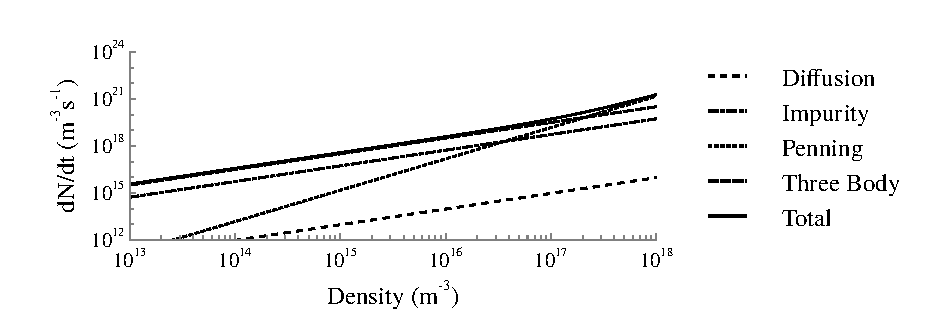
\includegraphics{./chapters/metastables/figures/decay.eps}
  \caption{Comparison of the decay rates for various processes at 0.3 Torr as a
  function of metastable density.}
  \label{fig:decay}
\end{figure}
illustrates the aforementioned decay processes at 0.3 Torr, for a variety of
metastable densities. The rate constants for these processes were obtained from
the study by Deloche et al.~\cite{Deloche1976} and the work of Pouvesle et
al.~\cite{Pouvesle1988} (specifically for the rate of Penning ionization of
nitrogen impurities). The gas impurities were assumed to be nitrogen, and the
mole fraction was assumed to be 80 ppm, as was estimated in
chapter~\ref{chp:experiment}.

As can be seen, the dominant loss mechanism above metastable densities of
$2\times10^{17}$ m$^{-3}$ was Penning ionization between two metastable atoms.
Below this density, three-body process responsible for dimer formation was
dominant. However, the three-body process scales with the square of the neutral
gas pressure. As a result, this loss mechanism quickly overtakes all others as
the pressure is increased. Therefore, the exponential dependence of the decay at
higher pressures is not representative of any change in the importance of
Penning ionization between metastables, but rather the increasing importance of
three-body collisions. This indicates that the effectiveness of the metastable
population as a long-lived source of ionization decreases as the pressure is
increased.

From figures~\ref{fig:decay} and~\ref{fig:long}, it can be seen that the decay
curves are well matched by the exponential functions at lower line-integrated
metastable densities. As a result, it is possible to use the fitting functions
to estimate the pre-pulse metastable densities as a function of pressure. These
values are compiled in table~\ref{tbl:prepulse}.
\begin{table}
  \centering
  \caption{Listing of the extrapolated, pre-pulse line-integrated metastable 
  densities, and decay coefficients as a function of pressure.}
  \begin{tabular}{lll}
    \toprule
    Pressure (Torr) & Integral Density (m$^{-2}$) & Decay Constant (s$^{-1}$) \\
    \midrule
    0.3  & $1.34\times10^{14}$ & $4.23\times10^3$ \\
    0.5  & $3.36\times10^{14}$ & $3.47\times10^3$ \\
    1.0  & $4.29\times10^{14}$ & $3.65\times10^3$ \\
    2.0  & $2.60\times10^{14}$ & $4.48\times10^3$ \\
    3.0  & $3.94\times10^{13}$ & $6.47\times10^3$ \\
    4.0  & $5.04\times10^{12}$ & $8.73\times10^3$ \\
    8.0  & $7.08\times10^{6}$  & $2.20\times10^4$ \\
    16.0 & $4.74\times10^{0}$  & $3.56\times10^4$ \\
    \bottomrule
  \end{tabular}
  \label{tbl:prepulse}
\end{table}
For the conditions under which it was possible to measure the pre-pulse
line-integrated densities, these extrapolations show reasonable agreement
(within a factor of two). This implies that the other extrapolated pre-pulse
values are likely accurate. The decay constants are about an order of magnitude
larger than those recorded by Phelps and Molnar \cite{Phelps1953} at similar
pressures. This almost certainly reflects the impact of the impurities present
in the system. Figure~\ref{fig:decay} shows that impurities are a moderate
contributor to the decay of the metastable atoms even at low pressures. If the
impurities remain a fixed fraction of the helium in the system, then their
impact can be expected to rise as the operating pressure is increased. The
measurements and calculations of Deloche et al.~\cite{Deloche1976} also give
lower decay constants, emphasizing this conclusion. Their work also showed a
relatively consistent proportionality between the electron density and
metastable density (on the order of one for every ten). Therefore, the results
presented above may be used as a rough estimate of the line-integrated electron
densities in the system.

\section{Summary}
A laser diode-based absorption spectroscopy experiment was set up to observe the
development of the \acs{rpnd} on short (0-1700 ns) and long (0-700 $\mu$s) time
scales. The measurements on the short time scale provide some of the only
detailed measurements of the \acs{rpnd} during its development. The design of
the system and post-processing software carefully accounted for plasma-related
noise, background emissions, and laser drift. The absorption spectra model
showed excellent agreement with measured spectra and the matching algorithm
produced consistent and reliable results almost all cases.

Temperature measurements from the Doppler broadening of the absorption spectra
showed no appreciable gas heating at any operating pressure. These results
contrast with some measurements made in molecular \acs{rpnd}s where a variety of
additional mechanisms are available to transfer kinetic energy from electrons to
heavier species.

The line-integrated density results suggest that the plasma is axially uniform
across the tube at lower pressures, however the 8.0 and 16.0 Torr conditions
show significant attenuation with distance from the anode. This may represent a
geometric limit to the use of similar \acs{rpnd}s in material processing. The
dominant metastable loss mechanism at low pressures and short time periods is
Penning ionization between metastables. However, losses are eventually dominated
by three-body dimer formation for all cases. Peak metastable generation is
optimized at 4.0 Torr. However, the peak pre-pulse metastable densities are
optimized at 1.0 Torr. This also corresponds with the maximum measured energy
deposition from chapter~\ref{chp:experiment}.

These measurements provide an important foundation upon which to develop a more
encompassing idea of how the \acs{rpnd} develops. Specifically, the generation
of the metastable atoms is related to a number of other plasma parameters,
including: electron density, electron temperature, \acs{eedf}, and electric
field. Many of these quantities are related in a variety of ways, both subtle
and obvious. Provided a sufficiently detailed model, it should be possible to
capture these relationships, and use the measured metastable densities to infer
the evolution of these quantities as well as other excited states in the system.
